\section{Analysis}
\label{sec:analysis}

\begin{table*}[t]
\caption{Isolating the alias-instead-of-delete rule. Replacing the alias operation by
deletion in the sensitive-and-relevant cell, with everything else held fixed, costs a large
and significant amount wherever the anchor is itself a sensitive value (multi-entity,
single-hop, two-hop) and nothing where it is not (topical variants, no anchor). The
two-hop column is the clearest case: the reference answer is present in the context in
$96.3\%$ of cases under the delete variant, and F1 is nevertheless $0.0000$, because the
account that identifies the record has been removed.}
\label{tab:ablation_alias}
\centering\small
\setlength{\tabcolsep}{6pt}
\begin{tabular}{lrrrr}
\toprule
Benchmark & \textsc{DARK} & delete variant & $\Delta$ & 95\% CI \\
\midrule
extension, all ($2{,}728$)     & 0.4937 & 0.3142 & $+0.1795$ & $[+0.1643,+0.1945]$ \\
\quad multi-entity ($1{,}500$) & ---    & ---    & $+0.3273$ & $[+0.3040,+0.3513]$ \\
\quad needle ($1{,}228$)       & ---    & ---    & $-0.0010$ & $[-0.0105,+0.0086]$ (n.s.) \\
main set ($112$)               & 0.6366 & 0.5205 & $+0.1161$ & $[+0.0446,+0.1875]$ \\
LongBench topical ($300$)      & 0.3516 & 0.3503 & $+0.0013$ & $[-0.0002,+0.0042]$ (n.s.) \\
LongBench single-hop ($300$)   & 0.9607 & 0.1674 & $+0.7933$ & $[+0.7430,+0.8426]$ \\
LongBench two-hop ($300$)      & 0.6733 & 0.0000 & $+0.6733$ & $[+0.6200,+0.7256]$ \\
\bottomrule
\end{tabular}
\end{table*}


\subsection{Why redundancy ordering fails here}
A redundancy ordering keeps the record that carries the answer about half the time. On the
$2{,}728$-case extension the redundancy-only rule retains it in $47.5\%$ of cases ($56.0\%$
multi-entity, $37.2\%$ needle); protecting the anchor line raises this to $57.6\%$, and
routing on the record block reaches $100\%$. The question has to be asked in its own terms
because aggregate F1 hides it: every arm here produces an answer, and the score does not say
whether the record that grounds it is still in the prompt.

The two failure rates say different things. Multi-entity survival sits either side of the
budget cut, which is what an uninformative ordering produces: the score does not know which
record the question is about, so it keeps the right one about half the time. Needle survival
is \emph{below} the cut, and there the ordering is worse than uninformative. The answer in a
needle case is a field value that recurs across distractor records, so the record holding it
looks like a typical record and inherits no priority from the score. Protecting the anchor
line repairs this for needle cases---retention rises from $37.2\%$ to $59.9\%$---but the line
it protects is not the line that carries the answer, which is why the repair stops short of
$100\%$ rather than reaching it.

Figure~\ref{fig:survival} breaks the same question down by budget, by source, and by what the
retention is worth. Panel (a) follows the answer record across the budget curve: the two arms
that route on the record block hold it in $100\%$ of the 112 cases from $r=0.50$ upward and in
$56.2\%$ at $r=0.10$, while the two arms that only protect the anchor line stay between
$24.1\%$ and $77.7\%$ across the whole range. Panel (b) sets survival against F1 for the
$2{,}728$-case extension. Survival accounts for a good part of the ordering but not all of it:
the delete variant keeps the answer record in $100\%$ of cases and still scores $0.0000$ on
multi-entity cases, because the record it keeps no longer says which account it belongs to. The
dissociation is not an artefact of the aggregate: panel (c) repeats the comparison within each
of the six sources, and the block-level rule holds the answer in every case of every source
while the redundancy-only rule falls to $16.7\%$ on \arm{toolmem\_raw}. Panel (d) shows what
that retention is worth per source; the one source where the block rule is behind, by
$-0.065$, is the one where the redundancy-only arm retains $83.3\%$ and the two are
effectively tied.

\begin{figure*}[t]
\centering
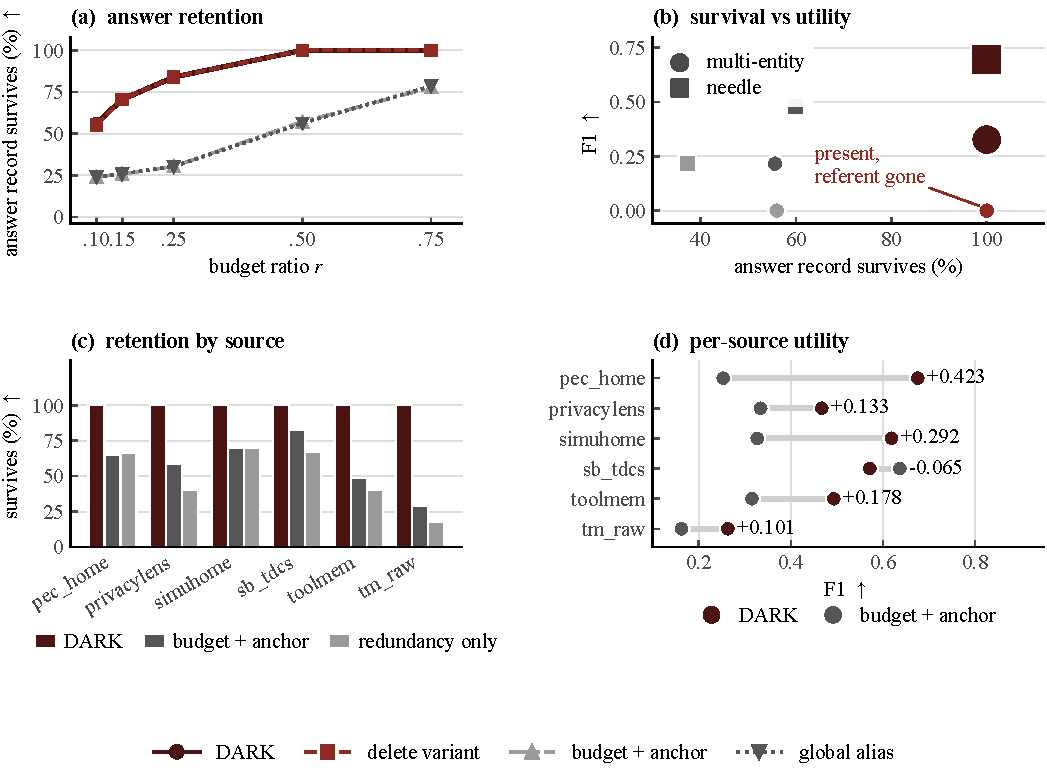
\includegraphics[width=\textwidth]{figures/fig2_diagnostic.pdf}
\caption{Answer retention and what it does not explain. (a) Fraction of the 112 benchmark
cases in which the record carrying the reference answer survives compression, as the budget
varies. \textsc{DARK} and the delete variant coincide almost exactly: the
alias-instead-of-delete rule does not change \emph{which} units survive. (b) Survival against
F1 on the $2{,}728$-case extension; circles are multi-entity cases and squares are needle
cases, and the four arms are the redundancy-only rule, the same rule with the anchor line
protected, \textsc{DARK}, and the delete variant. The delete variant sits at $100\%$ survival
and $0.0000$ F1 on multi-entity cases: the information is in the prompt and cannot be
located. (c) Retention within each source at
$r=0.50$. (d) Per-source F1, \textsc{DARK} against the anchor-protected arm, with the
paired difference printed at each row.}
\label{fig:survival}
\end{figure*}

\subsection{The layout the rule depends on}

The routing rule rests on two structural claims, and until now both were quoted as survival
percentages rather than measured. We measured them from the case text alone: segment each
excerpt on its record markers, take the first line that mentions the queried entity and the
first line that carries the reference answer, and report their distance
(Figure~\ref{fig:structure}). No model is involved, so the measurement is independent of the
reader.

Both claims hold, and the split between the two case kinds is sharper than the aggregate
suggested. On the $1{,}500$ multi-entity cases the anchor and the answer always land in the
same block---$1{,}500$ of $1{,}500$---and never on the same line: the anchor sits on the
private-contact lines and the answer inside the record line beneath it, two or five lines
away in $87\%$ of cases. On the $1{,}228$ needle cases the answer is again inside the
anchor's block in every case by annotation---an independent text-based re-derivation recovers
$99.8\%$, the two exceptions being cases where the answer string also occurs in an earlier
block---but in $56\%$ of them it shares the anchor's line.

This asymmetry decides which of the two design choices carries the gain, and the two are not
interchangeable. Widening the protected region from the anchor \emph{line} to the whole
\emph{block} lifts F1 on both families---$0.4802$ to $0.6473$ on needle, $0.2165$ to $0.3487$
on multi-entity---because in both the answer lives in the block and not always on the line.
Switching the operation from deletion to aliasing, by contrast, pays only where the anchor is
itself the protected value: $0.0000$ to $0.3487$ on multi-entity, and $0.6416$ to $0.6473$ on
needle, where the record identifier that the question names is not a canary and survives
either way.

\begin{figure*}[t]
\centering
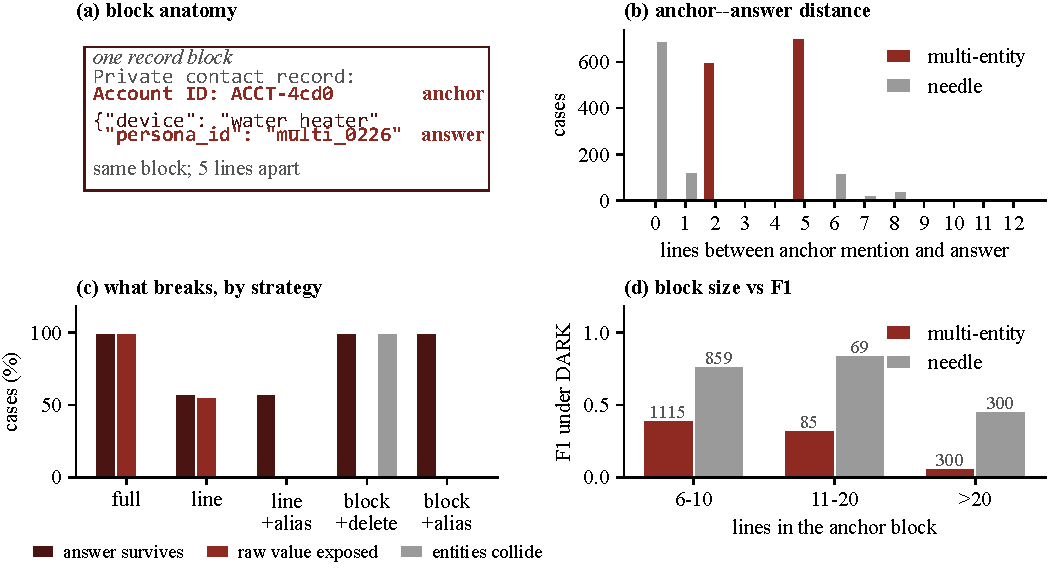
\includegraphics[width=\textwidth]{figures/fig_structure.pdf}
\caption{The structure the rule depends on, measured from the case text without a model.
(a)~Inside one record block the anchor sits on the private-contact line and the answer inside
the record line, five lines below it. (b)~The anchor-answer line distance per case kind: the
multi-entity cases are never closer than two lines, the needle cases usually share the line.
(c)~Five retention strategies scored on the only three things that can break---the answer
span, exposure of the raw protected value, and collision of distinct entities onto one
surface token. Reading left to right, each step of the design changes exactly one of the
three columns. (d)~DARK's F1 against the size of the block it has to keep; numbers above the
bars are case counts. Once the anchor block exceeds twenty lines the rule degrades, which is
where the fallback window stops being able to carry the answer.}
\label{fig:structure}
\end{figure*}

Panel~(c) is what separates the three design choices, because reading it left to right each
step moves exactly one column and leaves the other two where they were. Replacing the raw
text with aliases at a fixed selection takes raw exposure from $55.4\%$ to $0\%$ while answer
retention stays at $57.6\%$. Widening the protected region from the line to the block takes
answer retention from $57.6\%$ to $100\%$ while exposure stays at $0\%$. Deleting instead of
aliasing inside that block leaves both columns untouched---the answer still survives and
nothing is exposed---and instead takes collision from $0\%$ to $100\%$, because every
sensitive value becomes the same string and the reader can no longer tell which record the
question is about. That single column is the whole difference between F1 $0.4937$ and
$0.3142$, and it is why the operation and not merely the region is load-bearing.

Panel~(d) marks the boundary. Keeping the block is enough while the block is compact; past
roughly twenty lines DARK's F1 on multi-entity cases falls from $0.370$ to $0.257$, and on
needle cases from $0.724$ to $0.395$, because a large block spends the budget on itself and
the answer drifts outside the fallback window. The rule does not fail gracefully here: it
still emits a prompt within budget, and the loss appears only in the score.

\subsection{Protecting the anchor line is not enough}
A natural repair forbids dropping units that mention the queried entity. It does not close the
gap, and where it helps it helps for the wrong reason. Overall retention moves from $47.5\%$
to $57.6\%$, but the two families behave differently: multi-entity retention is unchanged
($56.0\%$ to $55.6\%$), while needle retention rises from $37.2\%$ to $59.9\%$. Needle cases
improve because the anchor there is the record identifier, which happens to share the record
with the answer far more often than the account line does. The reason the repair stops short
of $100\%$ is layout: the line carrying the account identifier and the line carrying the
answer are different units in $100\%$ of multi-entity cases and in $65.4\%$ of needle cases.
Preserving the identifier preserves the pointer, not the content.

The repair becomes effective one level up. The excerpt is laid out in record blocks, and the
block containing the anchor mention also contains the answer in every case of the
benchmark, as its annotations record. Constraining the block instead of the line restores answer
retention to $100\%$ on both families without consulting the answer key. This is the
measurement that motivates the routing rule: the relevant region is a block, not a unit.

\subsection{The operation and the interface}
Replacing the alias operation by deletion costs the task exactly where the design says it
should. Holding the context construction fixed, the difference is large and significant where
the anchor is itself a sensitive value: $+0.3273$ on multi-entity cases, $+0.7933$ on the
single-hop variant, $+0.6733$ on the two-hop variant. Where no anchor exists---the topical
variant, whose questions name no entity---it is $+0.0013$ and not significant. On the needle
family, whose anchor is a non-sensitive record identifier, it is $-0.0010$ and not
significant.

\begin{figure*}[t]
\centering
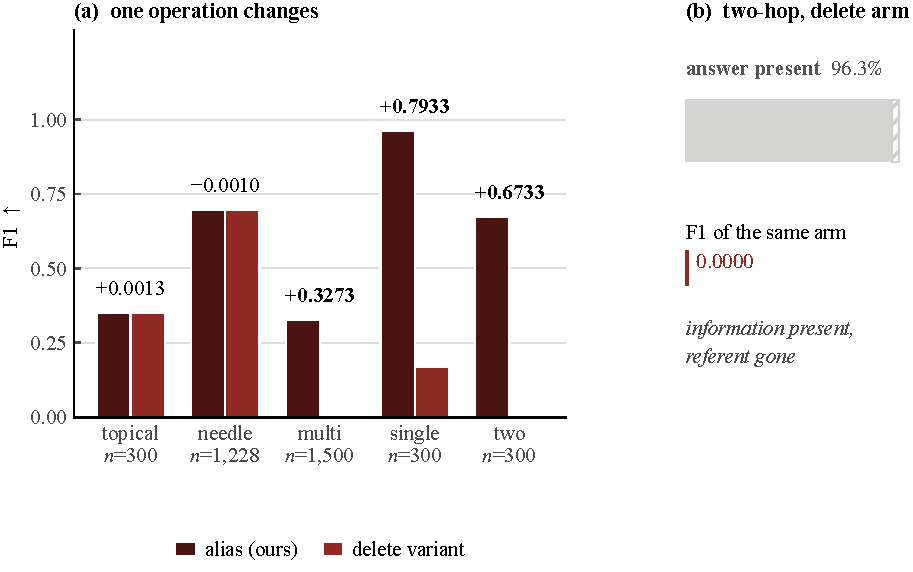
\includegraphics[width=\textwidth]{figures/fig3_alias.pdf}
\caption{Replacing the alias operation by deletion, with the context construction otherwise
unchanged, on five settings. (a) The difference concentrates exactly where the anchor is a
protected value and vanishes where it is not; labels give the paired difference of the two
bars and a star marks an interval that excludes zero. (b) Distribution of the paired per-case
difference for the three settings where the operation matters. The mass sits at both ends
because a case is either answered or not, and the mean gain is largest on the single-hop
variant. (c) In the two-hop variant the answer is still in the prompt after $96.3\%$ of the
deletions, and F1 is zero.}
\label{fig:aliasdelete}
\end{figure*}

% Fig.6 —— 两个真实案例的定性对比（预测为模型实际输出）
\definecolor{anchorbg}{HTML}{DCE4E6}
\definecolor{failbg}{HTML}{F0E4E2}
\definecolor{okbg}{HTML}{E4EAE7}

\begin{figure*}[t]
\centering

\begin{minipage}[t]{0.47\textwidth}
\centering
{\small\bfseries (a) two-hop: the answer sits behind a chain}\\[3pt]
{\scriptsize\itshape Q: which device does account \texttt{ACCT-5f31} operate?}\\[4pt]
\begin{flushleft}\ttfamily\scriptsize\setlength{\parskip}{1.5pt}
\textcolor{black!45}{164}\ \ \colorbox{anchorbg}{\strut account ACCT-5f31} belongs to \colorbox{anchorbg}{\strut user U-5a675c}\\
\textcolor{black!45}{\dots}\\
\textcolor{black!45}{170}\ \ \colorbox{anchorbg}{\strut user U-5a675c} operates device \underline{sensor\_422708\_15}
\end{flushleft}
\vspace{3pt}
{\scriptsize\itshape after aliasing, both links keep a name:}\\[3pt]
\begin{flushleft}\ttfamily\scriptsize
\colorbox{anchorbg}{\strut account [ACCT-A]} belongs to \colorbox{anchorbg}{\strut user [USER-B]}\\
\colorbox{anchorbg}{\strut user [USER-B]} operates device \underline{sensor\_422708\_15}
\end{flushleft}
\end{minipage}\hfill
\begin{minipage}[t]{0.47\textwidth}
\centering
{\small\bfseries (b) multi-entity: the answer looks like a distractor}\\[3pt]
{\scriptsize\itshape Q: which persona id is recorded for account \texttt{ACCT-447f...}?}\\[4pt]
\begin{flushleft}\ttfamily\scriptsize\setlength{\parskip}{1.5pt}
\textcolor{black!45}{07}\ \ \{``device'': ``dehumidifiers'',\\
\phantom{07}\ \ \ ``id'': \underline{``multi\_0166\_00''}, \dots\}\\
\textcolor{black!45}{08}\ \ Private contact record:\\
\textcolor{black!45}{09}\ \ Contact email: contact.e67e...\\
\textcolor{black!45}{11}\ \ \colorbox{anchorbg}{\strut Account ID: ACCT-447fa54ac66d}
\end{flushleft}
\vspace{3pt}
{\scriptsize\itshape the target account is the eleventh of sixteen,}\\
{\scriptsize\itshape and its record is shaped like every other record.}
\end{minipage}

\vspace{7pt}
\resizebox{\textwidth}{!}{%
\begin{tabular}{lcccc}
\toprule
 & \arm{full} & \arm{alias} & \arm{delete} & \textsc{DARK} \\
\midrule
(a)\ \ two-hop, \texttt{lbc-hotpotqa-0000} & \colorbox{okbg}{sensor\_422708\_15} & \colorbox{okbg}{sensor\_422708\_15} & \colorbox{failbg}{UNKNOWN} & \colorbox{okbg}{sensor\_422708\_15} \\
(b)\ \ multi-entity, \texttt{multi-0032} & \colorbox{failbg}{UNKNOWN} & \colorbox{okbg}{multi\_0166\_00} & \colorbox{failbg}{UNKNOWN} & \colorbox{okbg}{multi\_0166\_00} \\
\bottomrule
\end{tabular}}

\caption{Two cases where the routing changes the answer, with the predictions the reader
actually produced. In (a) the question names an account that reaches the answer only through
a user identifier six records later; deleting either link leaves the answer present but
unreachable, and the model returns \textsc{unknown}. In (b) the answer sits in one of sixteen
near-identical account records, so the uncompressed prompt \emph{also} fails---here the
distractor structure, not the budget, is what defeats the reader---while both aliasing arms
answer correctly. Shaded spans mark the names that keep a chain addressable.}
\label{fig:cases}
\end{figure*}


Figure~\ref{fig:cases} shows the two failure modes at the level of a single case, with the
predictions the reader actually produced.

The two-hop column is the most informative single result in this paper. Under the delete
variant the reference answer is present in the context in $96.3\%$ of cases, so GIC is
essentially saturated, and F1 is $0.0000$. The information is in the prompt; the reader
cannot use it, because the identifier saying which record it belongs to has been removed.
String-presence metrics do not detect this failure, which is why we report task quality and
leakage as separate endpoints rather than as one utility score.

\paragraph{The question side.}
Aliasing the context without rewriting the question produces a prompt whose halves use
different names for the same entity. We measured both settings over the full $2{,}728$ cases
with the pipeline otherwise unchanged; $\Delta$ is the original-question score minus the
rewritten one, so a negative value is what the rewrite is worth. On the subset where the
question names a protected entity, dropping the rewrite takes the score to exactly zero.

\begin{center}\small
\setlength{\tabcolsep}{4pt}
\resizebox{\columnwidth}{!}{%
\begin{tabular}{lcccc}
\toprule
Benchmark & rewritten & original & $\Delta$ & 95\% CI \\
\midrule
extension ($2{,}728$)        & 0.4937 & 0.3132 & $-0.1806$ & $[-0.195,-0.167]$ \\
\quad multi-entity ($1{,}500$) & 0.3273 & 0.0000 & $-0.3273$ & $[-0.351,-0.303]$ \\
\quad needle ($1{,}228$)       & 0.6970 & 0.6957 & $-0.0014$ & $[-0.005,+0.002]$ (n.s.) \\
\bottomrule
\end{tabular}}
\end{center}

The damage is confined to the cases where the question names a protected entity. On
multi-entity excerpts the unrewritten prompt scores exactly $0.0000$: the question asks about
\texttt{ACCT-4cd0} while every record offers \texttt{[ACCT-A]}, so no record can be matched
and the reader cannot answer no matter what survives compression. On needle excerpts, where
the question names a record identifier rather than an account, the step is worth $0.0014$ and
the interval includes zero. The other alias arms behave the same way: \arm{alias\_budget}
loses $0.0444$ overall and \arm{alias\_budget\_link} $0.1272$, the latter falling by $0.2314$
on multi-entity and by exactly $0.0000$ on needle.

The step costs nothing in privacy---leakage is $0\%$ in both conditions---so its entire value
is recovered utility. We therefore treat the pair $(q',P)$ rather than $P$ alone as the object
of study, and verify the mapping before generation.

\subsection{What the answer key would add}
A rule allowed to read the reference answer gains a great deal from it. On the full
$2{,}728$ cases, handing the answer span to four redundancy-based arms raises F1 by
$0.157$ to $0.305$, and the gain is largest for the two anchor-protected arms---the arms used
in the main comparison.

\begin{center}\small
\setlength{\tabcolsep}{4pt}
\resizebox{\columnwidth}{!}{%
\begin{tabular}{lcc}
\toprule
Arm & $\Delta$ F1 from answer key $\uparrow$ & 95\% CI \\
\midrule
BC  & $+0.1571$ & $[+0.144,+0.171]$ \\
ALB & $+0.1731$ & $[+0.159,+0.188]$ \\
BCL & $+0.3046$ & $[+0.287,+0.322]$ \\
ABL & $+0.3042$ & $[+0.287,+0.323]$ \\
\bottomrule
\end{tabular}}
\end{center}

The two groups gain in different places, and the split is diagnostic. On needle cases the
redundancy-only arms gain $0.348$ and $0.349$, because the answer value repeats across
distractor records and knowing it tells the rule which copy to keep. On multi-entity cases
those same arms gain almost nothing ($0.001$ and $0.029$), while the anchor-protected arms
gain $0.368$ and $0.367$---precisely the reverse. Each arm is helped where it was previously
blind.

\textsc{DARK} reports every number in this paper without that input, because a deployed
pipeline holds no reference answer. Stating the size here fixes the scale of what the rule
obtains from the question alone: the referential benefit is reachable at inference time, not
only in an evaluation that still holds the key. The oracle is not a privacy repair either:
the anchor-protected arm forwards a protected value in $0\%$ of cases with or without it, and
the compress-only arm in $55.7\%$ with it against $55.4\%$ without.

\subsection{Sensitivity and scope}
Section~\ref{sec:method-budget} left the traversal direction of the refill queue as an
empirical choice. Running both directions end to end settles it at one boundary and leaves it
open everywhere else.

\begin{center}\small
\setlength{\tabcolsep}{4pt}
\resizebox{\columnwidth}{!}{%
\begin{tabular}{lcccc}
\toprule
Benchmark & increasing & decreasing & $\Delta$ & 95\% CI \\
\midrule
extension ($2{,}728$) & 0.4937 & 0.4832 & $-0.0106$ & $[-0.028,+0.007]$ \\
main set ($112$)      & 0.6366 & 0.5844 & $-0.0522$ & $[-0.124,+0.019]$ \\
topical ($300$)       & 0.3516 & 0.3172 & $-0.0344$ & $[-0.090,+0.020]$ \\
single-hop ($300$)    & 0.9607 & 0.9719 & $+0.0111$ & $[-0.008,+0.032]$ \\
two-hop ($300$)       & 0.6733 & 0.0167 & $-0.6567$ & $[-0.712,-0.599]$ \\
\bottomrule
\end{tabular}}
\end{center}

For four of the five rows the interval includes zero: away from the boundary the order of
refill units does not decide whether the answer survives. The two-hop benchmark \emph{is} the
boundary. There the answer sits six sentences from the anchor, outside the fallback window,
so whether it is present at all is decided by which units refill admits, and keeping the
repetitive ones retrieves it ($0.6733$ against $0.0167$). We read this as a property of this
data---the anti-correlation between redundancy and answer-bearing measured at the start of
this section---rather than as a guarantee, which is why
Section~\ref{sec:discussion} proposes widening the relevant region instead of relying on the
ordering.

\paragraph{Rule-based compressors on records.}
A 2026 line compresses without a model call at all: deterministic lexical rules delete filler, contractions, stop words and function words, then lemmatise what remains~\cite{chokshi-lexical-2026}. We ran its most aggressive preset over all $2{,}728$ cases on CPU. It realises $5{,}817$ context tokens against our $4{,}146$ and the uncompressed $8{,}482$, so it compresses less than we do, and it scores $0.3696$ F1 against our $0.4937$, a paired difference of $-0.1242$ $[-0.1462,-0.1016]$ at $100\%$ leakage against our $0\%$. The mechanism is visible in the text. The rules strip braces and rename keys---\texttt{device} to \texttt{twist} in one case---so the number of parseable JSON objects in the corpus falls from $273{,}209$ of $299{,}408$ ($91.2\%$) to zero, and the reader receives a word salad in which the record boundaries that anchor the question no longer exist. A compressor tuned on prose is not a compressor for records.

\paragraph{Where the rule applies.}
The three LongBench-derived variants locate the boundary.

\begin{center}\small
\setlength{\tabcolsep}{4pt}
\resizebox{\columnwidth}{!}{%
\begin{tabular}{lrrr}
\toprule
Variant & \arm{full} & \arm{alias} & \textsc{DARK} \\
\midrule
topical ($300$)     & 0.4181 & 0.4074 & 0.3516 \\
single-hop ($300$)  & 0.9889 & 0.9197 & 0.9607 \\
two-hop ($300$)     & 0.0967 & 0.7078 & 0.6733 \\
\bottomrule
\end{tabular}}
\end{center}

On the topical variant the questions name no entity, so there is nothing to route on: the
rule degenerates to global aliasing plus redundancy ordering and loses $0.0665$ against the
uncompressed prompt. That variant lies outside what this rule addresses, and we report it as
such rather than as a failure of the mechanism.

The two-hop row carries a second observation. Without sanitization the raw prompt scores
$0.0967$; with global aliasing it scores $0.7078$. The identifiers in this variant are long
hexadecimal strings differing in a few characters, so replacing them with short distinct
tokens makes the task \emph{easier} for the reader. Privacy and utility move in the same
direction here, a useful counterpoint to the usual framing, though the effect belongs to the
identifier surface form rather than to the routing rule.
